%-------------------------------------------------------------------------------
%	CAPITOLO 24
%-------------------------------------------------------------------------------

\chapter{I batocchi delle campane}
Verso il 1870 serpeggiava in paese ancora la lotta dei liberali contro il partito papalino, che aveva il suo esponente nei preti. I preti erano i più forti di numero, perché contavano sull'elemento femminile, sui contadini, i quali mal sopportavano le ultime schioppettate della guerra d'indipendenza nazionale, e la leva nuovamente introdotta.\\
\indent Per gente che fugge il rumore e bada solamente ai propri interessi, le vecchie idee, solo perché contrarie al nuovo ordine erano un vangelo, la sacrestia e la chiesa el tempio della ribellione contro le novità. Bastava un rintocco di campana per radunare il popolo tutto a dispetto dell'elemento liberale. \\
\indent Si era giunti al carnevale, l'elemento liberale voleva scialarsela\footnote{Godersela, spassarsela}, ballare anche la seconda mezzanotte del martedì grasso che cadeva in Quaresima. Dal canto della chiesa come contromisura erano state chiamate ed in funzione le sacre missioni.\\
\indent Questo fu il colmo! Le ragazze morigerate allora disertarono i festini, schivarono i fidanzati o come suol dirsi i filarini, che forse avevano pensato per un anno di avere nelle braccia le loro belle, almeno nel ballo.\\
\indent Maledette campane! Oltre che stordire gli abitué della piazza chiamavano alla chiesa ed alle prediche il bel sesso, e popolo alla mattina, pomeriggio, sera, con relative confessioni, comunioni... per tenerle sempre in devozione ed in santità lontano dai peccati. Figurate l'ossessione degli irati filarini-liberali a... spasso per la forzata disoccupazione.
Il vecchio campanaro \index[Personaggi]{Barabisa (campanaro)}Barabisa come sempre, va a suonare l'Ave Maria del giorno, ma tira, tira, credeva di avere perduto la forza e di non suonare le campane. Bisognò che rischiarasse la mente sonnolenta per convincersi... di essere ancora lui... in forza.\\
\indent Che era? Che non era?\\
\indent Avevano, nella notte, portato via i batocchi delle campane!\\
\indent La voce si diffuse in un baleno, tutti furono mobilitati alla ricerca affannosa dei sacri batocchi in ogni angolo. Si pescavano anche nelle sabbie del fiume, e un colpevole che assistiva a questa curiosa pesca... si mordeva... e brontolava... <<è non sono mica lì>>.\\
\indent Finalmente, dopo tre giorni il detto \index[Personaggi]{Il Dio Scalzo}Dio Scalzo, un fanatico portastendardo delle confraternite, un poveraccio, arrivò a pescare tra le acque e sabbie del fiume i rubati batocchi e trionfò in nome della fede, in odio ai nemici ed ai due paoli al giorno per la ricerca\footnote{Trovati i batacchi delle campane, esultò anche per i soldi guadagnati per la ricerca}.\\
\indent Per quel carnevale... fu una quaresima per gli innamorati\footnote{Mentre le campane erano fuori uso, i ragazzi potevano festeggiare il carnevale liberamente}.
 
 
 
 \begin{figure}[htb]
    \centering
    \vspace{-0.2cm}
    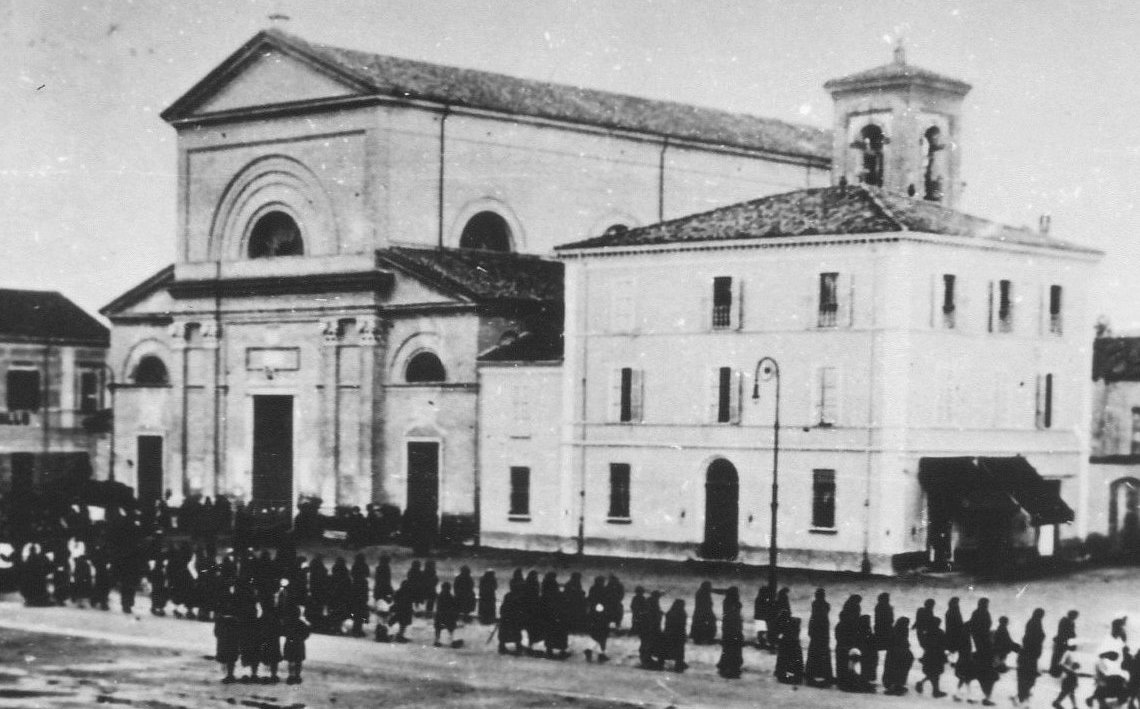
\includegraphics[width=0.9\textwidth]{chiesa}
    \caption[Arcipretale Santa Maria]{La chiesa \textbf{Arcipretale Santa Maria}\index[Luoghi]{Arcipretale Santa Maria} in Piazza \index[Luoghi]{Piazza Vincenzo Monti}Monti con a fianco la canonica, fotografata durante una processione.\label{fig:chiesa}}
    \vspace{-0.7cm}
\end{figure}






















%